\documentclass{standalone}
\usepackage{tikz}
\usepackage{ctex,siunitx,ninecolors}
\setCJKmainfont{Noto Serif CJK SC}
\usepackage{tkz-euclide}
\usepackage{amsmath}
\usetikzlibrary{patterns, calc}
\usetikzlibrary {decorations.pathmorphing, decorations.pathreplacing, decorations.shapes,}
\begin{document}
\small
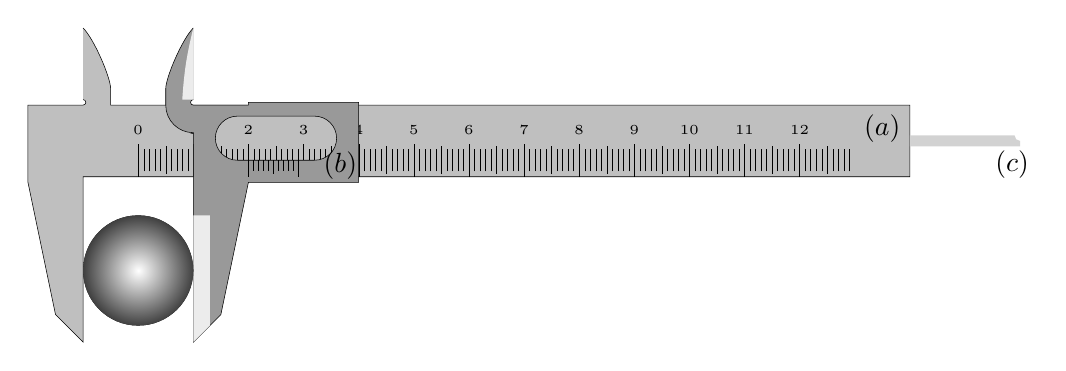
\begin{tikzpicture}[>=stealth,scale=0.7]
  \fill[lightgray,draw=black,very thin](-1,2.4)..controls(-0.8,2.2)and(-0.5,1.5)..(-0.5,1.3)--(-0.5,1.0)--(14,1.0)node[below left,text=black]{$(a)$}--(14,-0.3)--(-1,-0.3)--++(0,-3)--++(-0.5,0.5)--++(-0.5,2.4)--(-2,1.0)--(-1.0,1.0)arc(-90:90:0.05);
  \foreach \x in {0,1,...,12}
  {
    \draw[ultra thin](\x,-0.3)--++(0,0.6)node[above]{\tiny \x};
    \draw[ultra thin](\x+0.5,-0.25)--++(0,0.5);
    \foreach \y in {1,2,3,4,6,7,8,9}
    {
      \draw[ultra thin](\x+0.1*\y,-0.2)--++(0,0.4);
    }
  }
  \fill[lightgray!70](14,0.25)--(16,0.25)--(16,0.35)node[below,text=black,xshift=-0.1cm]{$(c)$}arc(270:180:0.1)--(14,0.45)--cycle;
  \begin{scope}[xshift=2cm]
    \fill[gray!80,draw=black,very thin,even odd rule](-1,2.4)..controls(-1.2,2.2)and(-1.5,1.5)..(-1.5,1.3)--(-1.5,1.0)arc(180:270:0.5)--(-1,-3.3)--++(0.5,0.5)--++(0.5,2.4)--++(2,0)node[above left,text=black,xshift=.1cm,yshift=-0.09cm]{$(b)$}--++(0,1.45)--++(-2.0,0)--++(0,-0.05)--++(-1.0,0)arc(270:90:0.05)
    (-0.2,0)--(1.2,0)arc(-90:90:0.4)--++(-1.4,0)arc(90:270:0.4)
    ;
    \foreach \x in {1,2,3,4,6,7,8,9}
    {
      \draw[ultra thin] (\x*0.09,0)--++(0,-0.2);
    }
    \draw[ultra thin] (0,0)--++(0,-0.3);
    \draw[ultra thin] (0.9,0)--++(0,-0.3);
    \draw[ultra thin] (0.45,0)--++(0,-0.25);
    \fill[lightgray!30](-1,2.4)to[bend right=5](-1.2,1.1)--(-1,1.1);
    \fill[lightgray!30](-1,-3.3)--++(0.3,0.3)--++(0,2)--++(-0.3,0);
  \end{scope}
  \fill[inner color=white,outer color=darkgray](0,-2)circle(1);
\end{tikzpicture}
\end{document}